\documentclass{article}
\usepackage[a4paper,margin=1in]{geometry}
\usepackage{amsmath, amssymb, amsthm}
\usepackage{xspace}
\usepackage{needspace, etoolbox}
\usepackage{url}

\usepackage{mdframed}
\usepackage{hyperref}
\usepackage{cleveref}
\usepackage{thm-restate}

\usepackage{tikz}
\usepackage{tikz-cd}
\usetikzlibrary{arrows.meta,positioning,shapes.geometric} % note: geometric instead of misc
\usetikzlibrary{backgrounds}

\tikzset{
  port/.style     = {circle, draw, inner sep=0pt, minimum size=6pt},
  junction/.style = {diamond, aspect=2, draw, fill=gray!20, inner sep=0pt, minimum size=8pt},
  sum/.style      = {circle, draw, inner sep=0pt, minimum size=10pt, font=\footnotesize},
  wire/.style     = {-{Latex}},
  faint/.style    = {gray!50, dashed},
  labelstyle/.style = {font=\small}
}

% llbracket rrbracket
\usepackage{stmaryrd}

\usepackage[font=small,labelfont=bf]{caption}
\captionsetup[figure]{width=.85\linewidth,justification=raggedright,singlelinecheck=false}


\usetikzlibrary{fit, backgrounds, calc}

% ---------- Minimal linear-algebraic scaffolding ----------
\newcommand{\K}{\mathbb{K}}                  % base field
\newcommand{\N}{\mathbb{N}}                  % natural numbers
\newcommand{\vect}[1]{\mathbf{#1}}           % bold vectors
\newcommand{\mat}[1]{\mathbf{#1}}            % bold matrices
\newcommand{\id}{\mat{I}}                    % identity
\newcommand{\zeros}{\mat{0}}                 % zero matrix
\newcommand{\std}[1]{\vect{e}_{#1}}          % standard basis e_i
\newcommand{\arityin}{n}                     % input arity
\newcommand{\arityout}{m}                    % output arity

% Spaces of signals
\newcommand{\InSpace}{\K^{\arityin}}
\newcommand{\OutSpace}{\K^{\arityout}}

% Notation for routing matrices
\newcommand{\Rout}[2]{\mathsf{Rout}(#1,#2)}

% Define a new theorem style with extra space
\newtheoremstyle{spaced}
  {0pt}   % Space above (adjust to increase/decrease)
  {0pt}   % Space below (adjust to increase/decrease)
  {} % Body font (keep as default or change)
  {}        % Indent amount
  {\bfseries} % Theorem head font
  {}       % Punctuation after theorem head
  {1em}     % Space after theorem head
  {}        % Theorem head spec

\theoremstyle{spaced}

\mdfdefinestyle{myenvs}{%
  hidealllines=false,%
  nobreak=true, % comment this to allow breaking
}

\newmdtheoremenv[style=myenvs]{theorem}{Theorem}[section] % Main counter
\newmdtheoremenv[style=myenvs]{definition}[theorem]{Definition}
\newmdtheoremenv[style=myenvs]{lemma}[theorem]{Lemma}
\newmdtheoremenv[style=myenvs]{examples}[theorem]{Examples}
\newmdtheoremenv[style=myenvs]{proposition}[theorem]{Proposition}
\newmdtheoremenv[style=myenvs]{corollary}[theorem]{Corollary}


\newenvironment{reusable}[2]{%
        \restatable{#1}{#2}
        \label{#2}}
    {\endrestatable}

\title{Algorithmic Algebra}
\author{
Clément Michaud \\
Independent Researcher in AI\\
\texttt{clement.michaud34@gmail.com}
}
\date{March 2025}

\begin{document}

\maketitle

\begin{center}
\begin{minipage}{0.9\textwidth}
\small
\textbf{Abstract.} Describe what this paper is about.
\end{minipage}
\end{center}

\vspace{10pt}


\section{Introduction}

\subsection{Preliminary Definitions}

\paragraph{Notation.}
Throughout this work, we use bold lowercase letters (e.g.\ $\vect{x}, \vect{y}$) to denote vectors and bold uppercase letters (e.g.\ $\mat{C}, \mat{D}$) to denote matrices. 
This convention emphasizes their algebraic roles in expressions such as $\vect{y}=\mat{C}\vect{x}$, where the circuit matrix $\mat{C}$ acts linearly on the input vector $\vect{x}$ to produce an output signal $\vect{y}$. 
Scalars, by contrast, are written in regular (non-bold) type.

\begin{definition}[Field]
A \emph{field} is a set \(\K\) with operations \(+\) and \(\cdot\) such that
\((\K,+)\) is an abelian group with identity \(0\), 
\((\K\setminus\{0\},\cdot)\) is an abelian group with identity \(1\), 
and multiplication distributes over addition. 
Equivalently, a field is a commutative ring with \(1\) in which every nonzero element is invertible.
\end{definition}


\paragraph{Field of scalars.}
All signal values are taken in a fixed field~\(\K\), which provides the scalars for the underlying vector spaces. 
Typical choices include the real numbers~\(\mathbb{R}\), complex numbers~\(\mathbb{C}\), or a finite field~\(\mathbb{F}_q\), depending on the intended semantics of the circuit. 
The field structure ensures that vector addition and scalar multiplication satisfy the familiar algebraic laws required for linear operations.

\begin{definition}[Unit vector]
For each $n\in\N$, let $\mathbf{1}_{n}\in\K^{n}$ denote the \emph{unit vector of ones}, that is,
\[
\mathbf{1}_{n} := (1,1,\dots,1)^{\top}.
\]
It serves as a convenient shorthand for expressing uniform sums and column constraints in circuit matrices.
\end{definition}

\begin{definition}[Identity matrix]
For each \(n\in\N\), the \emph{identity matrix} of order \(n\) is the square matrix
\[
\id_n = (\,\delta_{ij}\,)_{1\le i,j\le n},
\quad\text{where}\quad
\delta_{ij} =
\begin{cases}
1, & \text{if } i=j,\\[2pt]
0, & \text{if } i\ne j.
\end{cases}
\]
It acts as the neutral element for matrix multiplication:
for every matrix \(\mat{A}\in\K^{m\times n}\) and every vector \(\vect{x}\in\K^{n}\),
\[
\id_n\vect{x} = \vect{x},
\qquad
\mat{A}\id_n = \mat{A},
\qquad
\id_m\mat{A} = \mat{A}.
\]
\end{definition}



\begin{definition}[Entrywise order on vectors]
For $\vect{u},\vect{v}\in\K^{n}$ we write $\vect{u}\le\vect{v}$ 
if and only if $u_i\le v_i$ for all $i=1,\dots,n$.
This defines the \emph{entrywise order} on $\K^{n}$.
\end{definition}

\subsection{Primitive Circuits}

\begin{definition}[Signals and circuit matrices]
Fix a field $\K$. For $n,m\in\N$, an \emph{input signal} is a vector $\vect{x}\in\K^{n}$ and an \emph{output signal} is a vector $\vect{y}\in\K^{m}$.
A \emph{circuit matrix} is any matrix $\mat{C}\in\K^{m\times n}$ acting on inputs by left multiplication $\vect{y}=\mat{C}\vect{x}$.
\end{definition}

\paragraph{Routing with fan-out.}
A routing specifies how input signals are directed to output ports.  
Each output can be driven by at most one input, ensuring there are no conflicting signal sources,  
while an input may be duplicated across several outputs, allowing fan-out.  
This behavior can be captured algebraically by a matrix of zeros and ones that encodes these connections.


\begin{definition}[Routing matrices with fan-out]
For $m,n\in\N$, define $\Rout{m}{n}\subseteq\{0,1\}^{m\times n}$ as the set of \emph{routing matrices} satisfying
\[
\Rout{m}{n}
=\bigl\{\mat{C}\in\{0,1\}^{m\times n}\ \bigm|\ 
\mat{C}^{\!\top}\mathbf{1}_{m}\ge \mathbf{0}_{n}\ \text{and}\ 
\mat{C}\mathbf{1}_{n}\le \mathbf{1}_{m}\bigr\}.
\]
Equivalently, every row of $\mat{C}$ contains at most one~$1$ (so each output receives at most one input), 
while any column may contain zero or more~$1$s (so an input may drive several outputs). 
For $\vect{x}\in\K^{n}$, the action $\vect{y}=\mat{C}\vect{x}$ duplicates input components according to these connections.
\end{definition}

\paragraph{Unconnected outputs.}
The condition $\mat{C}\mathbf{1}_{n}\le\mathbf{1}_{m}$ allows some rows of $\mat{C}$ to contain no ones at all.  
Such a row represents an output that is not connected to any input.  
Under matrix evaluation, this output receives the additive identity of the field~$\K$, producing a zero signal.  
Thus the formalism naturally accommodates circuits with unconnected outputs without requiring any special treatment.

%==================== Figure 1: Fan-out (1 → 2) ====================
\begin{figure}[t]
  \centering
  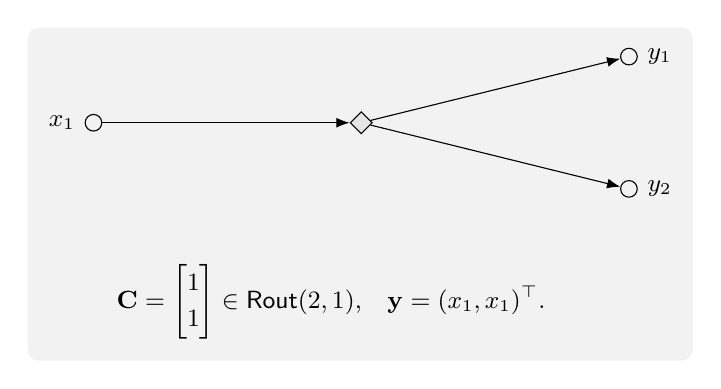
\begin{tikzpicture}[x=1.7cm, y=1.2cm, background rectangle/.style={fill=gray!10,rounded corners=4pt}, show background rectangle]
    % Ports
    \node[port,label={[labelstyle]left:$x_1$}] (x1) at (0,0) {};
    \node[port,label={[labelstyle]right:$y_1$}] (y1) at (4,0.7) {};
    \node[port,label={[labelstyle]right:$y_2$}] (y2) at (4,-0.7) {};
    % Mandatory connection point (junction) between input and outputs
    \node[junction] (j) at (2,0) {};
    % Wires
    \draw[wire] (x1) -- (j);
    \draw[wire] (j) -- (y1);
    \draw[wire] (j) -- (y2);
    % Inline matrix annotation (optional)
    \node[align=left,anchor=north west,font=\small] at (0.1,-1.4)
      {$\mat{C}=\begin{bmatrix}1\\[2pt]1\end{bmatrix}\in\Rout{2}{1}$,\quad
       $\vect{y}=(x_1,x_1)^\top$.};
  \end{tikzpicture}
  \caption{\textbf{Fan-out (1 input to 2 outputs).} A single input drives both outputs via an explicit junction node. This is allowed by the routing semantics (rows have at most one 1; columns may have multiple 1s).}
  \label{fig:fanout_1_to_2}
\end{figure}

%==================== Figure 2 : Unconnected output, single junction ====================
\begin{figure}[t]
  \centering
  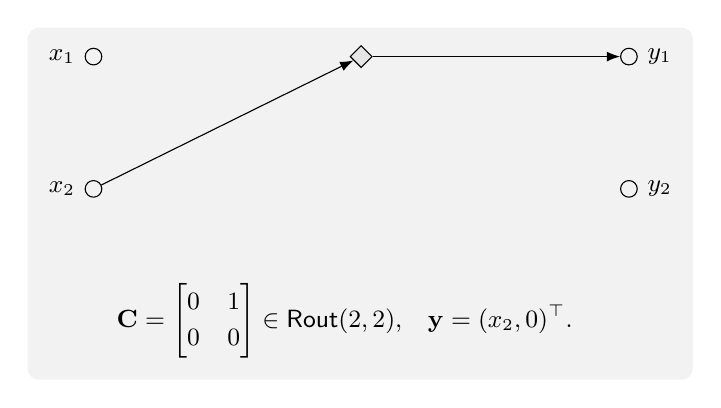
\begin{tikzpicture}[x=1.7cm, y=1.2cm, background rectangle/.style={fill=gray!10,rounded corners=4pt}, show background rectangle]
    % Inputs
    \node[port,label={[labelstyle]left:$x_1$}] (x1) at (0,0.7) {};
    \node[port,label={[labelstyle]left:$x_2$}] (x2) at (0,-0.7) {};
    % Outputs
    \node[port,label={[labelstyle]right:$y_1$}] (y1) at (4,0.7) {};
    \node[port,label={[labelstyle]right:$y_2$}] (y2) at (4,-0.7) {};
    % Single junction (connection point)
    \node[junction] (j) at (2,0.7) {};
    % Wires: only y1 is connected (x2 -> j -> y1). y2 is present but unconnected.
    \draw[wire] (x2) -- (j);
    \draw[wire] (j) -- (y1);
    % Annotation (optional)
    \node[align=left,anchor=north west,font=\small] at (0.1,-1.6)
      {$\mat{C}=\begin{bmatrix}0&1\\[2pt]0&0\end{bmatrix}\in\Rout{2}{2}$,\quad
       $\vect{y}=(x_2,0)^\top$.};
  \end{tikzpicture}
  \caption{\textbf{Unconnected output with a single connection point.} Only $y_1$ is driven (via the junction), while $y_2$ is present but has no incoming wire, yielding a zero signal.}
  \label{fig:unconnected_output_single_junction}
\end{figure}


%==================== Figure 3 (fixed): Merge via single junction ====================
\begin{figure}[t]
  \centering
  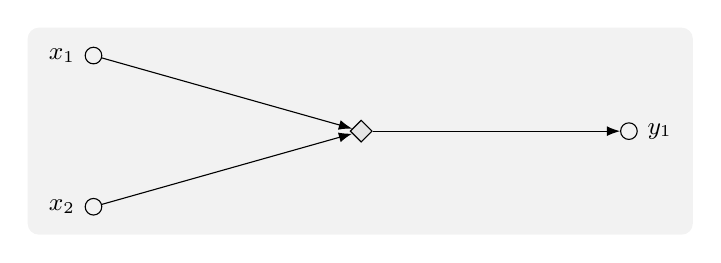
\begin{tikzpicture}[x=1.7cm, y=1.2cm, background rectangle/.style={fill=gray!10,rounded corners=4pt}, show background rectangle]
    % Inputs
    \node[port,label={[labelstyle]left:$x_1$}] (x1) at (0,0.8) {};
    \node[port,label={[labelstyle]left:$x_2$}] (x2) at (0,-0.8) {};
    % Output
    \node[port,label={[labelstyle]right:$y_1$}] (y1) at (4,0) {};
    % Single junction (connection point)
    \node[junction] (j) at (2,0) {};
    % Wires
    \draw[wire] (x1) -- (j);
    \draw[wire] (x2) -- (j);
    \draw[wire] (j) -- (y1);
  \end{tikzpicture}
  % Local caption formatting to prevent overfull/awkward spacing
  \captionsetup{width=.85\linewidth,justification=raggedright,singlelinecheck=false}
  \caption{\textbf{Merge drawn with a single connection point.}
  A single junction collects two inputs and feeds one output.
  In the pure-routing fragment this is illegal (multiple drivers per output); formally, it cannot be realized by any \(\mat{C}\in\Rout{1}{2}\) because rows must have at most one \(1\).}
  \label{fig:merge_single_junction_not_routing}
\end{figure}



\begin{definition}[Primitive circuit as routing]
Fix $m,n\in\N$. A \emph{primitive circuit} of arity $(n\!\to\! m)$ is a matrix $\mat{C}\in\Rout{m}{n}$. 
Its \emph{execution} (or \emph{evaluation}) on an input $\vect{x}\in\K^{n}$ is the output
\[
\llbracket \mat{C}\rrbracket(\vect{x})\;:=\;\mat{C}\vect{x}\in\K^{m}.
\]
Equivalently, each output coordinate copies exactly one input coordinate and no input is duplicated: if the unique $1$ in row $i$ of $\mat{C}$ is in column $j$, then $\bigl(\llbracket \mat{C}\rrbracket(\vect{x})\bigr)_{i}=x_{j}$.
\end{definition}

\begin{examples}
For $n=3,m=2$, 
$\displaystyle \mat{C}=\begin{bmatrix}0&1&0\\ 1&0&0\end{bmatrix}\in\Rout{2}{3}$.
For $\vect{x}=(x_1,x_2,x_3)^\top$, $\llbracket \mat{C}\rrbracket(\vect{x})=(x_2,x_1)^\top$.
\end{examples}

\paragraph{Identity circuits.}
Among all possible wirings, some circuits simply relay each input directly to the corresponding output without modification.  
Such circuits act as the identity transformation for their given arity: every signal passes through unchanged.  
They provide the neutral element for circuit composition—connecting any circuit before or after an identity circuit yields the same behavior.  
There is one such identity circuit for each arity \(n\), corresponding to an \(n\times n\) identity matrix.

\begin{definition}[Identity circuits]
For each \(n\in\N\), the \emph{identity circuit} of arity \(n\) is the routing matrix
\[
\id_n := \begin{bmatrix}
1 & 0 & \cdots & 0\\
0 & 1 & \cdots & 0\\
\vdots & \vdots & \ddots & \vdots\\
0 & 0 & \cdots & 1
\end{bmatrix} \in \Rout{n}{n}.
\]
For every input vector \(\vect{x}\in\K^{n}\),
\[
\llbracket \id_n \rrbracket(\vect{x}) = \id_n \vect{x} = \vect{x}.
\]
These identity circuits satisfy the compositional law
\[
\mat{C}\id_n = \mat{C}, \qquad
\id_m\mat{C} = \mat{C},
\]
for all \(\mat{C}\in\Rout{m}{n}\), expressing their role as the neutral elements of sequential composition.
\end{definition}


\subsection{Composition}

\paragraph{Composition of wiring circuits.}
Wiring circuits can be connected sequentially: the outputs of one circuit feed directly into the inputs of another.  
If the first circuit has arity \((n\!\to\!\ell)\) and the second \((\ell\!\to\! m)\), their composition yields a new circuit of arity \((n\!\to\! m)\).  
Because circuit execution corresponds to matrix multiplication, sequential composition is realized by multiplying the associated routing matrices.

\begin{definition}[Sequential composition of wiring circuits]
Let
\[
\mat{C}_1 \in \Rout{\ell}{n}
\quad\text{and}\quad
\mat{C}_2 \in \Rout{m}{\ell}.
\]
Their \emph{composition} is defined by
\[
\mat{C}_2 \circ \mat{C}_1 := \mat{C}_2 \mat{C}_1,
\]
that is, ordinary matrix multiplication in \(\K^{m\times n}\).
The result satisfies
\[
\llbracket \mat{C}_2 \circ \mat{C}_1 \rrbracket
 = \llbracket \mat{C}_2 \rrbracket \circ \llbracket \mat{C}_1 \rrbracket,
\]
and the identity matrix \(\id_n\) serves as a neutral element:
\[
\mat{C}\circ \id_n = \mat{C} = \id_m\circ \mat{C}.
\]
\end{definition}

\begin{proposition}[Closure and basic properties of composition]
Let $\Rout{m}{n}\subseteq\{0,1\}^{m\times n}$ denote routing matrices (each row has at most one $1$).
\begin{enumerate}
  \item \textbf{Closure.} If $\mat{C}_1\in\Rout{\ell}{n}$ and $\mat{C}_2\in\Rout{m}{\ell}$, then
  $\mat{C}_2\mat{C}_1\in\Rout{m}{n}$.
  \item \textbf{Associativity.} For any conformable $\mat{C}_1,\mat{C}_2,\mat{C}_3$ in routing sets,
  $(\mat{C}_3\mat{C}_2)\mat{C}_1=\mat{C}_3(\mat{C}_2\mat{C}_1)$.
  \item \textbf{Identities.} For each $n$, the identity matrix $\id_n\in\Rout{n}{n}$ and
  $\mat{C}\id_n=\mat{C}$ and $\id_m\mat{C}=\mat{C}$ for all $\mat{C}\in\Rout{m}{n}$.
\end{enumerate}
\emph{Proof sketch.}
(1) Write $(\mat{C}_2\mat{C}_1)_{ij}=\sum_{k=1}^{\ell} (\mat{C}_2)_{ik}(\mat{C}_1)_{kj}$.
Since row $i$ of $\mat{C}_2$ has at most one $1$, there is \emph{at most one} index $k^\ast$ with $(\mat{C}_2)_{ik^\ast}=1$.
Hence $(\mat{C}_2\mat{C}_1)_{ij}$ equals either $0$ (if no such $k^\ast$) or $(\mat{C}_1)_{k^\ast j}$.
Therefore row $i$ of $\mat{C}_2\mat{C}_1$ is either the zero row or a copy of some row of $\mat{C}_1$, and in either case it contains at most one $1$.
Also, all entries remain in $\{0,1\}$.
(2) Associativity is that of ordinary matrix multiplication.
(3) Follows from the defining properties of $\id_n$.
\qedhere
\end{proposition}

\begin{proposition}[Closure of routing matrices under composition]
If $\mat{C}_1\in\Rout{\ell}{n}$ and $\mat{C}_2\in\Rout{m}{\ell}$, then
$\mat{C}_2\mat{C}_1\in\Rout{m}{n}$.
\end{proposition}

\begin{proof}
By definition, $\mat{C}_1,\mat{C}_2$ are $\{0,1\}$-matrices with nonnegative entries and
\[
\mat{C}_1\mathbf{1}_n \le \mathbf{1}_\ell,
\qquad
\mat{C}_2\mathbf{1}_\ell \le \mathbf{1}_m
\quad\text{(entrywise).}
\]
Because left-multiplication by a nonnegative matrix is monotone, we have
\[
(\mat{C}_2\mat{C}_1)\mathbf{1}_n
=\mat{C}_2(\mat{C}_1\mathbf{1}_n)
\le \mat{C}_2\mathbf{1}_\ell
\le \mathbf{1}_m.
\]
Hence every row of $\mat{C}_2\mat{C}_1$ has sum at most $1$.

It remains to see that $\mat{C}_2\mat{C}_1$ is still $\{0,1\}$-valued.  
For each $i$, let $\vect{r}_i^\top:=\vect{e}_i^\top\mat{C}_2$ be the $i$-th row of $\mat{C}_2$.
Since $\mat{C}_2\mathbf{1}_\ell\le \mathbf{1}_m$, each $\vect{r}_i^\top$ is either the zero row or a standard basis row $\vect{e}_k^\top$ for some $k$.
Therefore
\[
\vect{e}_i^\top(\mat{C}_2\mat{C}_1)=\vect{r}_i^\top\mat{C}_1
\in \{\,\mathbf{0}^\top,\ \vect{e}_k^\top\mat{C}_1\,\}.
\]
In either case this row is $\{0,1\}$-valued, and (by the previous inequality) has sum at most $1$.
Thus $\mat{C}_2\mat{C}_1\in\Rout{m}{n}$.
\end{proof}


\begin{proposition}[Associativity of sequential composition]
Let $\mat{C}_1\in\Rout{\ell}{n}$, $\mat{C}_2\in\Rout{m}{\ell}$, and $\mat{C}_3\in\Rout{p}{m}$.
Then
\[
(\mat{C}_3\circ \mat{C}_2)\circ \mat{C}_1
\;=\;
\mat{C}_3\circ (\mat{C}_2\circ \mat{C}_1),
\qquad\text{i.e.}\qquad
(\mat{C}_3\mat{C}_2)\mat{C}_1=\mat{C}_3(\mat{C}_2\mat{C}_1).
\]
\end{proposition}

\begin{proof}
For all $i,j$,
\[
\bigl((\mat{C}_3\mat{C}_2)\mat{C}_1\bigr)_{ij}
=\sum_{r=1}^{\ell}\sum_{k=1}^{m} (\mat{C}_3)_{ik}(\mat{C}_2)_{kr}(\mat{C}_1)_{rj}
=\sum_{k=1}^{m}\sum_{r=1}^{\ell} (\mat{C}_3)_{ik}(\mat{C}_2)_{kr}(\mat{C}_1)_{rj}
=\bigl(\mat{C}_3(\mat{C}_2\mat{C}_1)\bigr)_{ij},
\]
where we used finiteness of the sums and the associativity/commutativity of addition together with associativity of scalar multiplication in the field $\K$.
Hence $(\mat{C}_3\mat{C}_2)\mat{C}_1=\mat{C}_3(\mat{C}_2\mat{C}_1)$.
Equivalently, for every $\vect{x}\in\K^{n}$,
\[
((\mat{C}_3\mat{C}_2)\mat{C}_1)\vect{x}
=\mat{C}_3(\mat{C}_2(\mat{C}_1\vect{x}))
=(\mat{C}_3(\mat{C}_2\mat{C}_1))\vect{x}.
\]
\end{proof}




% (Optional but handy) algebraic laws you can use later:
\begin{proposition}[Sequential and parallel structure, minimal form]
Let $\mat{C}_1\in\Rout{\ell}{n}$ and $\mat{C}_2\in\Rout{m}{\ell}$. Then $\mat{C}_2\mat{C}_1\in\Rout{m}{n}$ and
$\llbracket \mat{C}_2\mat{C}_1\rrbracket=\llbracket \mat{C}_2\rrbracket\circ\llbracket \mat{C}_1\rrbracket$.
Moreover, for block-diagonal $\mat{C}\in\Rout{m_1}{n_1}$ and $\mat{D}\in\Rout{m_2}{n_2}$,
$\mat{C}\oplus\mat{D}:=\begin{bmatrix}\mat{C}&\zeros\\ \zeros&\mat{D}\end{bmatrix}\in\Rout{m_1{+}m_2}{n_1{+}n_2}$ and
$\llbracket \mat{C}\oplus\mat{D}\rrbracket(\vect{x}\oplus\vect{z})=\llbracket \mat{C}\rrbracket(\vect{x})\oplus\llbracket \mat{D}\rrbracket(\vect{z})$.
\end{proposition}


\end{document}
